\chapter{Calcul de criticité en théorie de la diffusion}
\section{Criticité}
Le but est de voir s'il existe une solution à l'équation de diffusion dans un milieu fini 
homogène \textbf{sans} sources externes. C'est un effet la définition de la criticité, une 
réaction en chaîne auto-alimentée ce qui revient mathématiquement à tirer la source externe. Nous 
allons voir qu'il existe une solution en problème mais attention si l'on obtiens une solution 
sinusoïdale, le flux ne peut jamais être négatif ! Nous allons commencer par l'étude sans réflecteur

\subsection{Diffusion monocinétique}
Considérons un réacteur nu (pas de réflecteur) mais \textbf{avec} fissions (le terme "source" ici)
\begin{equation}
 - D\Delta \varphi (\bar r) + {\Sigma _a}\varphi (\bar r) = \nu {\Sigma _f}\varphi (\bar r)
\end{equation}
Il est toujours possible d'associer la CL précédemment vue, à savoir l'annulation du flux à la 
frontière extrapolée $\varphi(\bar r_s, \bar nd_s)=0$. Il s'agit d'un problème aux valeurs propres qui
peut s'écrire comme une équation d'Helmholtz
\begin{equation}
\Delta \varphi (\bar r) + {B^2}\varphi (\bar r) = 0
\end{equation}
où $\DS {B^2} = \frac{{\nu {\Sigma _f} - {\Sigma _a}}}{D}$. En en tire un ensemble dénombrable de 
valeurs propres, toutes de multiplicité unitaire
\begin{equation}
0 < B_o^2 < B_1^2 \le B_2^2 \leq \dots
\end{equation}
D'un point de vue physique, seul le mode fondamental est acceptable physiquement pour un flux car pas 
de changement de signe.\\

Il y a deux façons possible d'exprimer les valeurs propres du fondamental : la résolution du problème
aux valeurs propres et la définition du même facteur :
\begin{enumerate}
\item \textit{Buckling géomatrique}
\begin{equation}
B_g^2 = \frac{{ - \Delta {\varphi _o}}}{{{\varphi _o}}}
\end{equation}
\item \textit{Buckling matériel}
\begin{equation}
B_m^2 = \frac{{\nu {\Sigma _f} - {\Sigma _a}}}{D}
\end{equation}
\end{enumerate}
On peut voir $B_m$ comme la courbure du lobe.  On parle de criticité lorsque\\

\cadre{
\begin{equation}
B_g^2 = B_m^2
\end{equation}}\ \\

Le fondamental ne s'annulant pas, un certain nombre de fois la solution est toujours solution. La 
solution du flux n'est pas totalement déterminée mais la forme oui. Comme on fonctionne à une 
constante près, cela montre bien que la criticité ne donne \textbf{pas} la puissance ! 


\subsubsection{Problème dépendant du temps}
En introduisant les \textit{opérateurs de diffusion}
\begin{equation}
(J - K)\varphi (\bar r) = \nu {\Sigma _f}\varphi (\bar r) + D\Delta \varphi (\bar r) - {\Sigma _a}\varphi (\bar r)
\end{equation}
On peut en tirer un spectre de valeurs propres réelles
\begin{equation}
{\lambda _o} > {\lambda _1} \ge {\lambda _2} \ge \dots
\end{equation}
où $\DS {\lambda _i} = \nu {\Sigma _f} - {\Sigma _a} - DB_i^2$ et $B_i^2 \in \sigma ( - \Delta )$. \\

Si $\lambda_0$ est définie comme valant $\max_i\lambda_i$, elle correspond également à la valeur 
propre minimale de $(-\Delta)$. On associe alors $\varphi_0$ comme étant la fonction propres associée
à cette valeur propre, qui est positive sur tout le volume du réacteur.\\

En ré-écrivant l'équation, il est possible d'avoir tout les temps à gauche et la partie spatiale à 
droite 
\begin{equation}
\frac{1}{v}\frac{{\partial \varphi (\bar r,t)}}{{\partial t}} = (J - K)\varphi (\bar r,t)
\end{equation}
On peut alors appliquer la séparation des variables en développant sur la base des fonctions 
propres $\DS \varphi (\bar r,t) = \sum\limits_i    {c_i}(t){\varphi _i}(\bar r)$
\begin{equation}
\varphi (\bar r,t) = \sum\limits_i   {c_i}(0){\varphi _i}(\bar r){e^{{\lambda _i}vt}}
\end{equation}
Trois cas peuvent se présenter en fonction de la valeur propre
\begin{itemize}
\item[$\bullet$] $\lambda_0<0$ : état \textit{sous-critique}
\item[$\bullet$] $\lambda_0>0$ : état \textit{sur-critique}
\item[$\bullet$] $\lambda_0=0$ : état \textit{critique} avec $\varphi (\bar r,t)\overset{t\to+\infty}{\longrightarrow}{c_o}(0){\varphi _o}(\bar r)$
\end{itemize}
La seule solution possible pour le problème de criticité pour \textbf{toute} condition initiale est
\begin{equation}
{\lambda _i} = \nu {\Sigma _f} - {\Sigma _a} - DB_i^2\qquad\Longrightarrow\qquad {\lambda _o} = DB_m^2 - DB_g^2
\end{equation} 

\subsubsection{Criticité et facteur de multiplication}
Il doit exister un lien entre la criticité et la formule des six facteurs. Définissons $k_{eff}$ 
comme le rapport entre le nombre de neutrons produit et consommé (détruit). Proche de la criticité, 
on sait que $\varphi (\bar r) \approx {\varphi _o}(\bar r)$. On peut écrire $k_eff$ à l'aide des 
opérateurs de production $J$ et destruction $K$
\begin{equation}
{k_{eff}} = \frac{{J{\varphi _o}}}{{K{\varphi _o}}} = \frac{{\nu {\Sigma _f}}}{{{\Sigma _a} + D{B^2}}}
 = \frac{{\nu {\Sigma _f}}}{{{\Sigma _a}}}\frac{1}{{1 + {L^2}{B^2}}}
\end{equation}
Une autre façon de voir $\varphi_0$ via cette définition est de voir $\varphi_0$ comme une 
fonction fondamentales associée à la valeur propre $k_{eff}$
\begin{equation}
K\varphi  = \frac{1}{k}J\varphi 
\end{equation}
En oubliant le terme de fission rapide ($\varepsilon$), en supposant monoénergétique, sans 
probabilité de ralentissement et sans probabilité anti-trappe, on trouve\footnote{Dans un 
milieu infini ${k_\infty } = \frac{{\nu {\Sigma _f}}}{{{\Sigma _a}}} = \eta f$}\footnote{Il faudrait
ajouter les notes manuscrites, un dev. a été fait au tableau.}
\begin{equation}
{k_{eff}} = \frac{{\eta f}}{{1 + {L^2}{B^2}}} = \eta f{P_{th}}
\end{equation}
La \textbf{criticité est atteinte pour $k_{eff}=1$}. En ré-introduisant les facteurs laissés sur le
côté
\begin{equation}
{k_{eff}} = \eta \varepsilon pf.{P_{th}} = \frac{{\eta \varepsilon pf}}{{1 + {L^2}{B^2}}}
\end{equation}
Par identification
\begin{equation}
P_{th} = \dfrac{1}{1+L^2B^2}\qquad\text{ où }\quad B_m^2 = \frac{{\eta \varepsilon pf - 1}}{{{L^2}}}
\end{equation}
Il n'est pas étonnant de retrouver la valeur propre $B_m$ du buckling géométrique mais la criticité 
sera atteinte lorsqu'elle vaudra le buckling matériel.\\

Pour les sources indépendantes, l'idée est la même
\begin{equation}
(K - J)\varphi (\bar r) = Q(\bar r) = \sum\limits_i    {Q_i}{\varphi _i}(\bar r)
\end{equation}
On va pouvoir associer un développement en série du flux sur la même base (vecteurs propres) et voir
que par application de $(K-J)$ à ce flux on fait apparaître un facteur qui est l'inverse des 
$\lambda_i$
\begin{equation}
\varphi (\bar r) = \sum\limits_i   \frac{{{Q_i}}}{{DB_i^2 + {\Sigma _a} - \nu {\Sigma _f}}}{\varphi _i}(\bar r)
\end{equation}
Pour un cas légèrement sous-critique il existe une solution stationnaire possible à condition de se
rapprocher du fondamental. En première approximation, le premier terme sera dominant 
\begin{equation}
\varphi (\bar r) \approx \frac{{{Q_o}}}{{ - {\lambda _o}}}{\varphi _o}(\bar r) = \frac{{{Q_o}}}{{DB_o^2 + {\Sigma _a} - \nu {\Sigma _f}}}{\varphi _o}(\bar r)
\end{equation}
En première approximation, le flux est le fondamental multiplié par un coefficient qui reprend 
le fondamental de la source ainsi qu'un terme $1/-\lambda_0$. Un réacteur sous-critique est donc 
un amplificateur du mode fondamental de la source. C'est le genre de situation dans laquelle une 
source pourrait suppléer au définit de neutron que la réacteur est capable de fournir par rapport à 
ce qu'il consomme.

\subsection{Noyaux de modération}
Nous avons fait jusqu'ici un développement à un groupe où la variable énergie a été aplatie. Hélas, 
le cas monoénergétique est un peu scabreux et l'objectif est ici d'essayer d'améliorer le traitement 
de la variable énergie. 

\subsubsection{Définitions}
On définit le \textbf{noyau de ralentissement/modération} comme la densité de probabilité qu'un
neutron du à une fission en $\bar r_0$ est ralenti jusqu'à une énergie inférieure à $E$ en $\bar r$
\begin{equation}
P({\bar r_o} \to \bar r,E)
\end{equation}
La \textbf{densité de modération} est le nombre de neutrons par unité de volume et de temps qui sont 
ralentis en dessous de $E$ en $\bar r$ (voir chapitre 7)
\begin{equation}
q(\bar r,{E_{th}}) = \int\limits_V   P({\bar r_o} \to \bar r,{E_{th}})\nu {\Sigma _f}{\varphi _{th}}({\bar r_o})d{\bar r_o}
\label{eq:Ch4.1}
\end{equation}
où 
\begin{equation}
-D\Delta {\varphi _{th}}(\bar r) + {\Sigma _a}{\varphi _{th}}(\bar r) = q(\bar r,{E_{th}})
\end{equation}
Il s'agit de l'équation du \textit{flux thermique}. Le membre de gauche correspond à l'équation de 
diffusion à un groupe dans lequel la source $\nu\Sigma_f\varphi$ est remplacée par une densité 
de ralentissement (voir plus loin).\\
Justifions \eqref{eq:Ch4.1} : des neutrons vont être émis par unité de volume et de temps en quantité 
$\Sigma_f\varphi_{th}$. Le ralentissement permet d'aller dans la "seule zone" ou l'on peut avoir 
des fissions (toutes vont se faire aux énergies thermiques par hypothèses). A partir de ce nombre de
neutrons de fission par unité de volume et de temps, il y a une certaine probabilité que le neutron 
voit son énergie réduite en dessous de la limite définissant la zone thermique en migrant de $\bar 
r_0$ à $\bar r$.\\

Plutôt que de dire que tout neutron émis des fission est directement disponible, on considère à 
travers $P$ (noyau de ralentissement), une "fonction de transfert" qui fait passé les neutrons 
émis au point $\bar r_0$ avec une énergie élevée au point $\bar r$ avec une énergie possible.\\

Si l'on se place dans un réacteur de taille infinie on pourrait dire que peu importe le point 
$\bar r_0$ et $\bar r$ c'est la distance qui va définir l'expression de ce noyau : un produit de 
convolution apparaît et on peut utiliser les transformées de Fourier
\begin{equation}
({\Sigma _a} + D{B^2})\hat \varphi (B) = {(2\pi )^{3/2}}\hat P(B,{E_{th}})\nu {\Sigma _f}\hat \varphi (B)\qquad\Rightarrow\qquad {(2\pi )^{3/2}}\hat P(B,{E_{th}})\frac{{\nu {\Sigma _f}}}{{{\Sigma _a} + D{B^2}}} = 1\; \to \;B_m^2
\end{equation}
On obtient une expression qui permet d'obtenir la valeur de $B_m^2$. En "inversant" la précédente
expression 
\begin{equation}
\varphi (\bar r) = \int\limits_{}    A(\bar u).{e^{i{B_m}\bar u.\bar r}}d\bar u
\end{equation}
Ce qui est solution de $\Delta \varphi (\bar r) + B_m^2\varphi (\bar r) = 0$

\subsubsection{Solution dans un milieu fini}
Il faut comme condition supplémentaire que $B^2$ appartienne aux valeurs propres
de $(-\Delta)$ avec comme conditions aux limites la frontière extrapolée
\begin{equation}
{B^2} = B_o^2 = B_g^2
\end{equation}
Sans oublier la condition de criticité $B_m^2 = B_g^2$ où $B_m^2$ est solution de 
\begin{equation}
\underbrace{{(2\pi )^{3/2}}\hat P({B_m},{E_{th}})}_{\bar P(B_m,{E_{th}})}\frac{{\eta f}}{{1 + {L^2}B_m^2}} = 1
\end{equation}
Où l'on introduit $\bar{P}$ la probabilité de non fuite rapide (le slide 10 donne des exemples).

\newpage
\section{Réflecteurs}
\subsection{Introduction}
Cette fois-ci, le réacteur n'est plus nu mais entouré d'un réflecteur (matériau non fissible). Si 
l'on tient compte que le matériau peut renvoyer un certain nombre de neutrons vers la matière fissile 
on peut s'attendre à ce que moins de combustible soit nécessaire. En plus de renvoyé les neutrons, 
ils ont un rôle de ralentissement des neutrons (car bien souvent, leur composition est similaire à 
celle du modérateur). Le cas des réacteurs rapides ne sera ici pas considéré.


\subsection{Sauvetage réflectif}
\subsubsection{Modèle de diffusion mono-cinétique}
On va se retrouver avec la juxtaposition de deux zones de caractéristiques différentes mais 
supposées homogènes. Il faut résoudre l'équation de diffusion pour chacun de ces milieux et ensuite
relier ces deux solutions. Dans le noyau 
\begin{equation}
 - D\Delta \varphi (\bar r) + {\Sigma _a}\varphi (\bar r) = \nu {\Sigma _f}\varphi (\bar r)\qquad
 \Leftrightarrow\qquad \Delta \varphi (\bar r) + B_c^2\varphi (\bar r) = 0
\end{equation}
où $\DS B_c^2 = \frac{{\nu {\Sigma _f} - {\Sigma _a}}}{D} = \frac{{\eta f - 1}}{{{L^2}}} = \frac{{{k_\infty } - 1}}{{{L^2}}}$.\\

Dans le réflecteur, il n'y a pas de fission 
\begin{equation}
 - {D_R}\Delta \varphi (\bar r) + {\Sigma _{aR}}\varphi (\bar r) = 0\qquad\Leftrightarrow\qquad
\Delta \varphi (\bar r) - \frac{1}{{L_R^2}}\varphi (\bar r) = 0
\end{equation}
Il faut résoudre l'équation de diffusion dans chacune des $m$ zone. La solution dépendra de $2m$ 
constantes à déterminer à l'aide de la continuité, des CL, \dots On en tire un système d'équations 
non trivial qui n'a de solution non triviale que si son déterminant est nul, correspondant à la 
condition de criticité.\\

Considérons un noyau d'épaisseur $2a$ ainsi qu'un réflecteur d'épaisseur $b$ (longueur extrapolée). 
Par symétrie dans la résolution des équations de diffusion
\begin{equation}
\left\{\begin{array}{lll}
\varphi (x) &\DS={A\cos {B_c}x \;\;}&{0 \le x \le a}\\
\varphi (x) &\DS= {C\cosh \left( {\frac{x}{{{L_R}}}} \right) + E\sinh \left( {\frac{x}{{{L_R}}}} \right)}&{a \le x \le a + b}
\end{array}\right.
\end{equation}
En utilisant la continuité en $x=a$ et la condition aux limites (annulation du flux en $a+b$,la 
seule façon de faire est d'avoir un sinh car cosh ne s'annule jamais)
\begin{equation}
\left\{\begin{array}{lll}
\varphi (x) &\DS= {A\cos {B_c}x\quad \quad \quad \quad \quad \quad \;\;}&{0 \le x \le a}\\
\varphi (x) &\DS= {A\frac{{\cos {B_c}a}}{{\sinh {\textstyle{b \over {{L_R}}}}}}\sinh \left( {\frac{{a + b - |x|}}{{{L_R}}}} \right)}&{a \le x \le a + b}
\end{array}\right.
\end{equation}
Il faut que le courant soit continu entre le cœur et le réflecteur. Par continuité du courant, on en
tire l'\textit{équation de criticité} (souvent transcendantale)
\begin{equation}
D{B_c}\tan {B_c}a = \frac{{{D_R}}}{{{L_R}}}\coth \frac{b}{{{L_R}}}
\end{equation}
Notons que le coefficient $A$ restera indéterminé car la criticité ne dépend pas de ce par quoi on 
multiplie le flux.\\

La question légitime est de voir ce que l'on gagne en matière fissile. Pour un réacteur nu 
d'épaisseur $2a$, la criticité est atteinte lorsque $2{a_o} = \frac{\pi }{{{B_c}}}$. Les économies
dues aux réacteurs (le gain) s'expriment
\begin{equation}
\delta  = {a_o} - a = \frac{\pi }{{2{B_c}}} - a
\end{equation}
A condition de criticité, nous avons\footnote{C'était pas pour un nu ?}
\begin{equation}
\tan {B_c}\delta  = \frac{{D{B_c}}}{{{D_R}}}{L_R}\tanh \frac{b}{{{L_R}}}
\end{equation}
S'il n'y a pas trop de fission, $B_c\delta \ll 1$ 
\begin{equation}
\delta  \approx \frac{D}{{{D_R}}}{L_R}\tanh \frac{b}{{{L_R}}}
\end{equation}
Si on utilise le même matériau pour le réflecteur et le modérateur, $D$ est peu affecté par la 
proportion de carburant
\begin{equation}
\delta  \approx {L_R}\tanh \frac{b}{{{L_R}}}
\end{equation}
Faisons quelques approximations
\begin{itemize}
\item[$\bullet$] $b \ll L_r : \delta \approx b$ : si l'épaisseur du réflecteur est petite par rapport
à la longueur de diffusion, on gagne à peu près l'épaisseur du réflecteur.
\item[$\bullet$] $b \gg L_r : \delta \approx L_R$ : si l'épaisseur du réflecteur est beaucoup plus 
grande que la longueur de diffusion, on peut prendre l'épaisseur $L_r$ à l'interface avec le cœur 
pour donner les rétrodiffusions.
\end{itemize}


\subsection{Modèle à deux groupes}
On suppose le groupe 1 rapide et le second thermique. Dans le cœur, nous avons
\begin{equation}
\left\{\begin{array}{ll}
\DS - {D_1}\Delta {\varphi _1}(\bar r) + {\Sigma _{a1}}{\varphi _1}(\bar r) + {\Sigma _{s1}}{\varphi _1}(\bar r) &\DS= \nu {\Sigma _{f1}}{\varphi _1}(\bar r) + \nu {\Sigma _{f2}}{\varphi _2}(\bar r)\\
\DS- {D_2}\Delta {\varphi _2}(\bar r) + {\Sigma _{a2}}{\varphi _2}(\bar r) &\DS= {\Sigma _{s1}}{\varphi _1}(\bar r)
\end{array}\right.
\end{equation}
Dans le réflecteur, il n'y a pas de termes de fissions
\begin{equation}
\left\{\begin{array}{ll}
\DS- {D_{R1}}\Delta {\varphi _1}(\bar r) + {\Sigma _{R1}}{\varphi _1}(\bar r) &= 0\\
\DS- {D_{R2}}\Delta {\varphi _2}(\bar r) + {\Sigma _{R2}}{\varphi _2}(\bar r) &\DS= {\Sigma _{R1}}{\varphi _1}(\bar r)
\end{array}\right. 
\end{equation}
Travaillons en géométrie plane. Existe des solutions de type Helmholtz $- \Delta {\varphi _i} = {B^2}{\varphi _i}$. Pour que ce soit le cas, il faut que le déterminant de ce système soit nul. On va 
obtenir un $\varphi_1$ et un $\varphi_2$ associé aux $B_{1,2}^2$
\begin{equation}
\frac{{{\varphi _1}}}{{{\varphi _2}}} = \frac{{{D_2}{B^2} + {\Sigma _{a2}}}}{{{\Sigma _{s1}}}}
\end{equation}
Le slide 16 donne la solution de cette équation.\\


	\begin{wrapfigure}[12]{l}{5cm}
	\vspace{-5mm}
	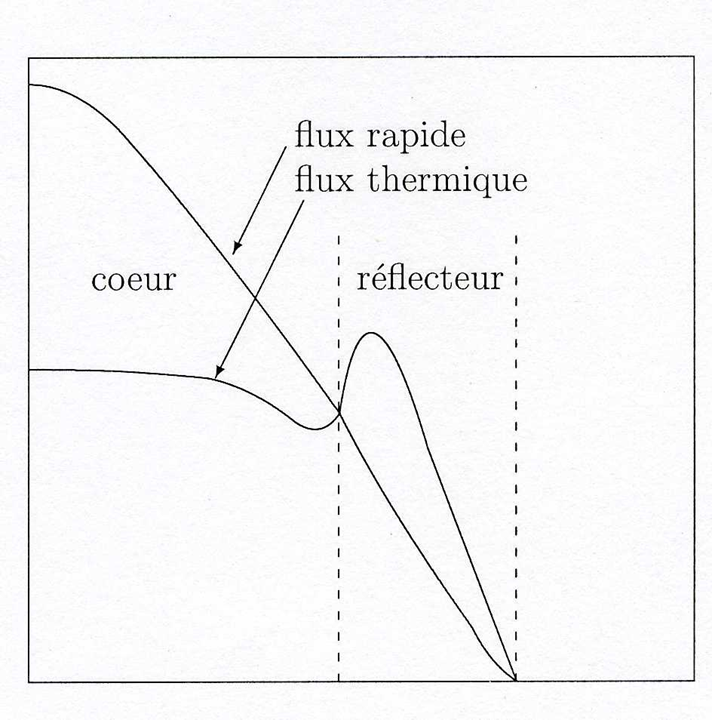
\includegraphics[scale=0.23]{ch4/image1.png}
	\captionof{figure}{ }
	\end{wrapfigure}
Ci-contre, on retrouve la solution en cosinus qui s'écrase bien jusqu'à l'annulation. Dans la 
partie thermique, la solution est plus constante dans le cœur et même si on retrouve au creux à 
proximité de la surface on retrouve un pic du flux dans le réflecteur car la longueur de diffusion
doit être d'environ la moitié du réacteur (car paquet de scattering qui va se faire en renvoyer 
une série de neutrons vers le coeur). on a également des neutrons produit grâce aux fissions 
renvoyés par le scattering(c'est dans le thermique que le retour vers le cœur se fait le plus).

























